% =============================================================================
%  Section for "Development": the heuristic used by A*
%  Uses only packages that are already in template.tex (amsmath, booktabs, graphicx, float, caption).
%  Put   % =============================================================================
%  Section for "Development": the heuristic used by A*
%  Uses only packages that are already in template.tex (amsmath, booktabs, graphicx, float, caption).
%  Put   % =============================================================================
%  Section for "Development": the heuristic used by A*
%  Uses only packages that are already in template.tex (amsmath, booktabs, graphicx, float, caption).
%  Put   % =============================================================================
%  Section for "Development": the heuristic used by A*
%  Uses only packages that are already in template.tex (amsmath, booktabs, graphicx, float, caption).
%  Put   \input{heuristic_section}   inside \section{Development}.
%  Bibliography: see references_ieee.tex (keys used here: aima3, hart1968, korf1997, culberson1998,
%  felner2004, holte2006, rokicki2013, cube20, korf1985, patel2014)
% =============================================================================

\subsection{The heuristic of A*}
\label{sec:heuristic}

\subsubsection{What A* needs from a heuristic}
A* expands first the node with the smallest value
\begin{equation}
    f(n) = g(n) + h(n),
\end{equation}
where $g(n)$ is the number of moves already made to reach $n$ and $h(n)$ is an estimation of the moves that are still missing to reach the solved cube \cite{aima3, hart1968}. A good introduction with visual examples can be found in \cite{patel2014}. The quality of $h$ decides how many nodes A* has to visit, and for the Rubik's Cube this is critical: the cube has $43{,}252{,}003{,}274{,}489{,}856{,}000$ reachable states \cite{korf1997, cube20}, every state has 18 possible moves (quarter and half turns of the six faces), and even the hardest cubes need 20 moves \cite{rokicki2013}.

Two properties are important \cite[pp.~94--95]{aima3}:
\begin{itemize}
    \item \textbf{Admissible:} $h(n) \le h^{*}(n)$, where $h^{*}(n)$ is the real number of moves needed from $n$. The heuristic never overestimates.
    \item \textbf{Consistent:} $h(n) \le c(n,a,n') + h(n')$ for every move $a$ that goes from $n$ to $n'$. Since every move costs $c = 1$, this means that $h$ changes at most by 1 after one move.
\end{itemize}
If $h$ is consistent (and therefore admissible), A* returns a shortest solution and a state never needs to be expanded twice \cite[p.~95]{aima3}. We need both properties in our program.

\subsubsection{First version of the heuristic and its problems}
Our first Python implementation used five small tables (explained below), each one storing information about only 4 cubies: two tables for 4 corners ($8\cdot7\cdot6\cdot5\cdot3^4 = 136{,}080$ states each) and three tables for 4 edges ($12\cdot11\cdot10\cdot9\cdot2^4 = 190{,}080$ states each), 842,400 entries in total. The heuristic was the maximum of the five values. It was correct, but it had two problems:
\begin{enumerate}
    \item \textbf{It is weak.} Each table ignores 8 of the 20 movable cubies, so its values are small. We measured the average value of $h$ over 20,000 random cubes and obtained only $6.45$ moves, while a typical random cube needs 17 or 18 moves \cite{cube20}. A weak heuristic makes A* expand a huge number of nodes.
    \item \textbf{It was built for 12 moves.} In the Python version only quarter turns existed. In this project we also use half turns ($F2$, $U2$, \dots), so there are 18 moves. A table built with quarter turns counts a half turn as 2 moves, so it can overestimate when the search counts it as 1 move, and the heuristic would stop being admissible. Every table must be built with exactly the same moves as the search.
\end{enumerate}

\subsubsection{Pattern databases}
The idea of a \textit{pattern database} (PDB) was introduced by Culberson and Schaeffer \cite{culberson1998} and it is also explained in our course book \cite[p.~106]{aima3}. We choose a part of the problem (for example, only the 8 corners of the cube and we ignore the edges). The number of moves needed to solve only that part can never be larger than the number of moves needed to solve the whole cube, so it is an admissible heuristic. Since that smaller problem has few states, we can solve \emph{all} its states in advance and save the answers in a table. During A*, computing $h(n)$ is only one table look-up.

The table is built with a breadth-first search that starts at the solved cube and applies the 18 moves again and again. The first time that the search reaches an arrangement of the pieces, the current depth is the distance of that arrangement to the solved state (the moves can be undone, so the distance from the solved cube is the same as the distance to it).

\subsubsection{Heuristic selected: 8 corners and two groups of 6 edges}
For the final version we use the heuristic of Korf \cite{korf1997}, who solved random cubes optimally with it. It uses three pattern databases:
\begin{enumerate}
    \item all 8 corners: $8! \cdot 3^7 = 88{,}179{,}840$ entries (the last corner twist is determined by the other seven, hence $3^7$);
    \item 6 edges (the first six edge cubies): $\frac{12!}{6!} \cdot 2^6 = 42{,}577{,}920$ entries;
    \item the other 6 edges: also $42{,}577{,}920$ entries.
\end{enumerate}
The heuristic is the maximum of the three values:
\begin{equation}
    h(n) = \max\bigl(h_{\text{corners}}(n),\; h_{\text{edges A}}(n),\; h_{\text{edges B}}(n)\bigr).
\end{equation}
Table~\ref{tab:pdb} shows the tables. Korf stored 4 bits per entry (82 MB in total); to keep our code simple we store one byte per entry (173 MB), which is small for our cluster. The tables are built once (about 12 seconds in our tests with 2 threads) and they are saved in a file for the next executions. As a check of our implementation, the average of the corner table is $8.764$, exactly the value reported by Korf \cite{korf1997}.

\begin{table}[H]
    \centering
    \renewcommand{\arraystretch}{1.3}
    \begin{tabular}{lrrrr}
        \toprule
        \textbf{Table} & \textbf{Entries} & \textbf{Memory} & \textbf{Average $h$} & \textbf{Max.\ $h$} \\
        \midrule
        8 corners          & 88,179,840 & 88.2 MB & 8.764 & 11 \\
        6 edges, set A     & 42,577,920 & 42.6 MB & 7.623 & 10 \\
        6 edges, set B     & 42,577,920 & 42.6 MB & 7.614 & 10 \\
        \bottomrule
    \end{tabular}
    \caption{Pattern databases used by A* (averages over all the entries of each table, measured with our program; Korf reports 8.764 for the corners and 7.668 for his 6-edge table \cite{korf1997}).}
    \label{tab:pdb}
\end{table}

\paragraph{Why the maximum and not the sum.} It would be tempting to add the three values to get a bigger heuristic, but this is not admissible for the cube: one turn of a face moves 4 corners \emph{and} 4 edges at the same time, so the same move would be counted in two tables. Adding values is only valid when the tables count different moves, as in additive pattern databases for sliding-tile puzzles \cite{felner2004}; the book also remarks that this does not work for the Rubik's Cube \cite[p.~107]{aima3}. Korf states that the only admissible way to combine corner and edge tables is to take the maximum \cite{korf1997}, and Holte et al.\ studied experimentally the use of several tables with the maximum \cite{holte2006}. We can also prove that the maximum keeps the two properties. Let $h_1, \dots, h_k$ be admissible and consistent heuristics and $h = \max_i h_i$:
\begin{itemize}
    \item \textit{Admissible:} for each $i$, $h_i(n) \le h^{*}(n)$, so $\max_i h_i(n) \le h^{*}(n)$.
    \item \textit{Consistent:} for each $i$, $h_i(n) \le 1 + h_i(n') \le 1 + h(n')$. Taking the maximum over $i$ on the left side gives $h(n) \le 1 + h(n')$.
\end{itemize}
Each table is itself consistent because it is the exact distance in a smaller version of the same puzzle, where one real move changes the pattern by at most one move. Our program also checks both properties in a self-test with thousands of random cubes.

\paragraph{How much better is it?} Figure~\ref{fig:hstrength} compares the average value of $h$ of the first version and of the final version over 20,000 random cubes for different scramble lengths. For a completely mixed cube the average goes from $6.45$ to $8.89$ moves (Korf reports $8.878$ \cite{korf1997}). It seems a small difference, but A* has to visit all the nodes with $f(n) = g(n) + h(n)$ smaller than the solution length, and the number of nodes grows exponentially with the depth, so every extra move of the heuristic removes a large part of the search. Korf also observed that the running time goes down approximately in proportion to the size of the tables \cite{korf1997}; our final tables have $173{,}335{,}680$ entries, about 206 times more than the 842,400 entries of the first version.

\begin{center}
    \begin{minipage}{0.9\textwidth}
        \centering
        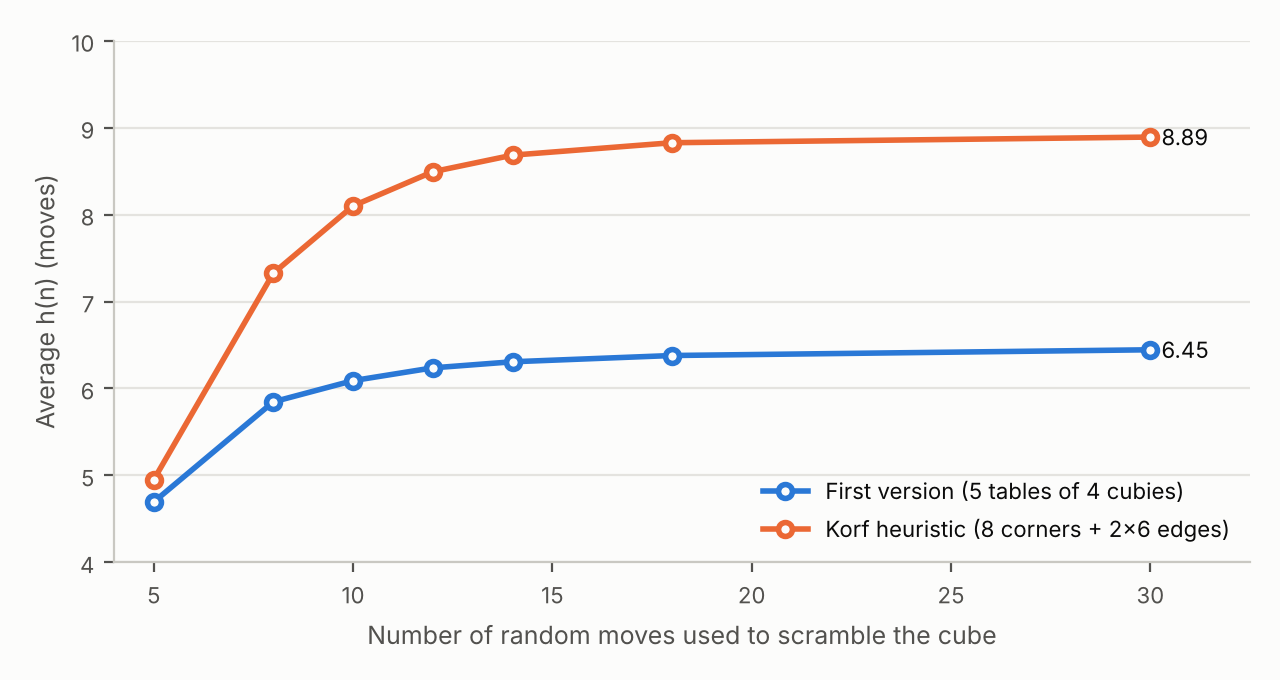
\includegraphics[width=\linewidth]{heuristic_strength.png}
        \captionof{figure}{Average value of $h$ for random cubes scrambled with different numbers of moves (20,000 cubes per point). Higher is better, as long as it is admissible.}
        \label{fig:hstrength}
    \end{minipage}
\end{center}

\subsubsection{Implementation details}
\begin{itemize}
    \item \textbf{Index of a table.} A pattern is converted to a number: the positions of the tracked cubies are encoded as a permutation number (Lehmer code), and the twists or flips of the cubies as a number in base 3 (corners) or base 2 (edges).
    \item \textbf{Open list.} Since every move costs 1, $f$ is always a small integer. Instead of a heap, the open list of our C++ A* is an array of lists, one list for every value of $f$. Inside a list, the newest node is expanded first (it has a larger $g$, so it is closer to the goal).
    \item \textbf{Redundant moves.} A face is never turned twice in a row, because two consecutive turns of the same face are always equal to one single move.
    \item \textbf{Memory.} Korf used IDA* \cite{korf1985}, a version that needs almost no memory, because A* stores every node it generates. We keep A* because it is the algorithm requested in this project, so we expect that for the deepest scrambles the memory of the cluster will be the limit; this will be analyzed in the Results.
\end{itemize}
   inside \section{Development}.
%  Bibliography: see references_ieee.tex (keys used here: aima3, hart1968, korf1997, culberson1998,
%  felner2004, holte2006, rokicki2013, cube20, korf1985, patel2014)
% =============================================================================

\subsection{The heuristic of A*}
\label{sec:heuristic}

\subsubsection{What A* needs from a heuristic}
A* expands first the node with the smallest value
\begin{equation}
    f(n) = g(n) + h(n),
\end{equation}
where $g(n)$ is the number of moves already made to reach $n$ and $h(n)$ is an estimation of the moves that are still missing to reach the solved cube \cite{aima3, hart1968}. A good introduction with visual examples can be found in \cite{patel2014}. The quality of $h$ decides how many nodes A* has to visit, and for the Rubik's Cube this is critical: the cube has $43{,}252{,}003{,}274{,}489{,}856{,}000$ reachable states \cite{korf1997, cube20}, every state has 18 possible moves (quarter and half turns of the six faces), and even the hardest cubes need 20 moves \cite{rokicki2013}.

Two properties are important \cite[pp.~94--95]{aima3}:
\begin{itemize}
    \item \textbf{Admissible:} $h(n) \le h^{*}(n)$, where $h^{*}(n)$ is the real number of moves needed from $n$. The heuristic never overestimates.
    \item \textbf{Consistent:} $h(n) \le c(n,a,n') + h(n')$ for every move $a$ that goes from $n$ to $n'$. Since every move costs $c = 1$, this means that $h$ changes at most by 1 after one move.
\end{itemize}
If $h$ is consistent (and therefore admissible), A* returns a shortest solution and a state never needs to be expanded twice \cite[p.~95]{aima3}. We need both properties in our program.

\subsubsection{First version of the heuristic and its problems}
Our first Python implementation used five small tables (explained below), each one storing information about only 4 cubies: two tables for 4 corners ($8\cdot7\cdot6\cdot5\cdot3^4 = 136{,}080$ states each) and three tables for 4 edges ($12\cdot11\cdot10\cdot9\cdot2^4 = 190{,}080$ states each), 842,400 entries in total. The heuristic was the maximum of the five values. It was correct, but it had two problems:
\begin{enumerate}
    \item \textbf{It is weak.} Each table ignores 8 of the 20 movable cubies, so its values are small. We measured the average value of $h$ over 20,000 random cubes and obtained only $6.45$ moves, while a typical random cube needs 17 or 18 moves \cite{cube20}. A weak heuristic makes A* expand a huge number of nodes.
    \item \textbf{It was built for 12 moves.} In the Python version only quarter turns existed. In this project we also use half turns ($F2$, $U2$, \dots), so there are 18 moves. A table built with quarter turns counts a half turn as 2 moves, so it can overestimate when the search counts it as 1 move, and the heuristic would stop being admissible. Every table must be built with exactly the same moves as the search.
\end{enumerate}

\subsubsection{Pattern databases}
The idea of a \textit{pattern database} (PDB) was introduced by Culberson and Schaeffer \cite{culberson1998} and it is also explained in our course book \cite[p.~106]{aima3}. We choose a part of the problem (for example, only the 8 corners of the cube and we ignore the edges). The number of moves needed to solve only that part can never be larger than the number of moves needed to solve the whole cube, so it is an admissible heuristic. Since that smaller problem has few states, we can solve \emph{all} its states in advance and save the answers in a table. During A*, computing $h(n)$ is only one table look-up.

The table is built with a breadth-first search that starts at the solved cube and applies the 18 moves again and again. The first time that the search reaches an arrangement of the pieces, the current depth is the distance of that arrangement to the solved state (the moves can be undone, so the distance from the solved cube is the same as the distance to it).

\subsubsection{Heuristic selected: 8 corners and two groups of 6 edges}
For the final version we use the heuristic of Korf \cite{korf1997}, who solved random cubes optimally with it. It uses three pattern databases:
\begin{enumerate}
    \item all 8 corners: $8! \cdot 3^7 = 88{,}179{,}840$ entries (the last corner twist is determined by the other seven, hence $3^7$);
    \item 6 edges (the first six edge cubies): $\frac{12!}{6!} \cdot 2^6 = 42{,}577{,}920$ entries;
    \item the other 6 edges: also $42{,}577{,}920$ entries.
\end{enumerate}
The heuristic is the maximum of the three values:
\begin{equation}
    h(n) = \max\bigl(h_{\text{corners}}(n),\; h_{\text{edges A}}(n),\; h_{\text{edges B}}(n)\bigr).
\end{equation}
Table~\ref{tab:pdb} shows the tables. Korf stored 4 bits per entry (82 MB in total); to keep our code simple we store one byte per entry (173 MB), which is small for our cluster. The tables are built once (about 12 seconds in our tests with 2 threads) and they are saved in a file for the next executions. As a check of our implementation, the average of the corner table is $8.764$, exactly the value reported by Korf \cite{korf1997}.

\begin{table}[H]
    \centering
    \renewcommand{\arraystretch}{1.3}
    \begin{tabular}{lrrrr}
        \toprule
        \textbf{Table} & \textbf{Entries} & \textbf{Memory} & \textbf{Average $h$} & \textbf{Max.\ $h$} \\
        \midrule
        8 corners          & 88,179,840 & 88.2 MB & 8.764 & 11 \\
        6 edges, set A     & 42,577,920 & 42.6 MB & 7.623 & 10 \\
        6 edges, set B     & 42,577,920 & 42.6 MB & 7.614 & 10 \\
        \bottomrule
    \end{tabular}
    \caption{Pattern databases used by A* (averages over all the entries of each table, measured with our program; Korf reports 8.764 for the corners and 7.668 for his 6-edge table \cite{korf1997}).}
    \label{tab:pdb}
\end{table}

\paragraph{Why the maximum and not the sum.} It would be tempting to add the three values to get a bigger heuristic, but this is not admissible for the cube: one turn of a face moves 4 corners \emph{and} 4 edges at the same time, so the same move would be counted in two tables. Adding values is only valid when the tables count different moves, as in additive pattern databases for sliding-tile puzzles \cite{felner2004}; the book also remarks that this does not work for the Rubik's Cube \cite[p.~107]{aima3}. Korf states that the only admissible way to combine corner and edge tables is to take the maximum \cite{korf1997}, and Holte et al.\ studied experimentally the use of several tables with the maximum \cite{holte2006}. We can also prove that the maximum keeps the two properties. Let $h_1, \dots, h_k$ be admissible and consistent heuristics and $h = \max_i h_i$:
\begin{itemize}
    \item \textit{Admissible:} for each $i$, $h_i(n) \le h^{*}(n)$, so $\max_i h_i(n) \le h^{*}(n)$.
    \item \textit{Consistent:} for each $i$, $h_i(n) \le 1 + h_i(n') \le 1 + h(n')$. Taking the maximum over $i$ on the left side gives $h(n) \le 1 + h(n')$.
\end{itemize}
Each table is itself consistent because it is the exact distance in a smaller version of the same puzzle, where one real move changes the pattern by at most one move. Our program also checks both properties in a self-test with thousands of random cubes.

\paragraph{How much better is it?} Figure~\ref{fig:hstrength} compares the average value of $h$ of the first version and of the final version over 20,000 random cubes for different scramble lengths. For a completely mixed cube the average goes from $6.45$ to $8.89$ moves (Korf reports $8.878$ \cite{korf1997}). It seems a small difference, but A* has to visit all the nodes with $f(n) = g(n) + h(n)$ smaller than the solution length, and the number of nodes grows exponentially with the depth, so every extra move of the heuristic removes a large part of the search. Korf also observed that the running time goes down approximately in proportion to the size of the tables \cite{korf1997}; our final tables have $173{,}335{,}680$ entries, about 206 times more than the 842,400 entries of the first version.

\begin{center}
    \begin{minipage}{0.9\textwidth}
        \centering
        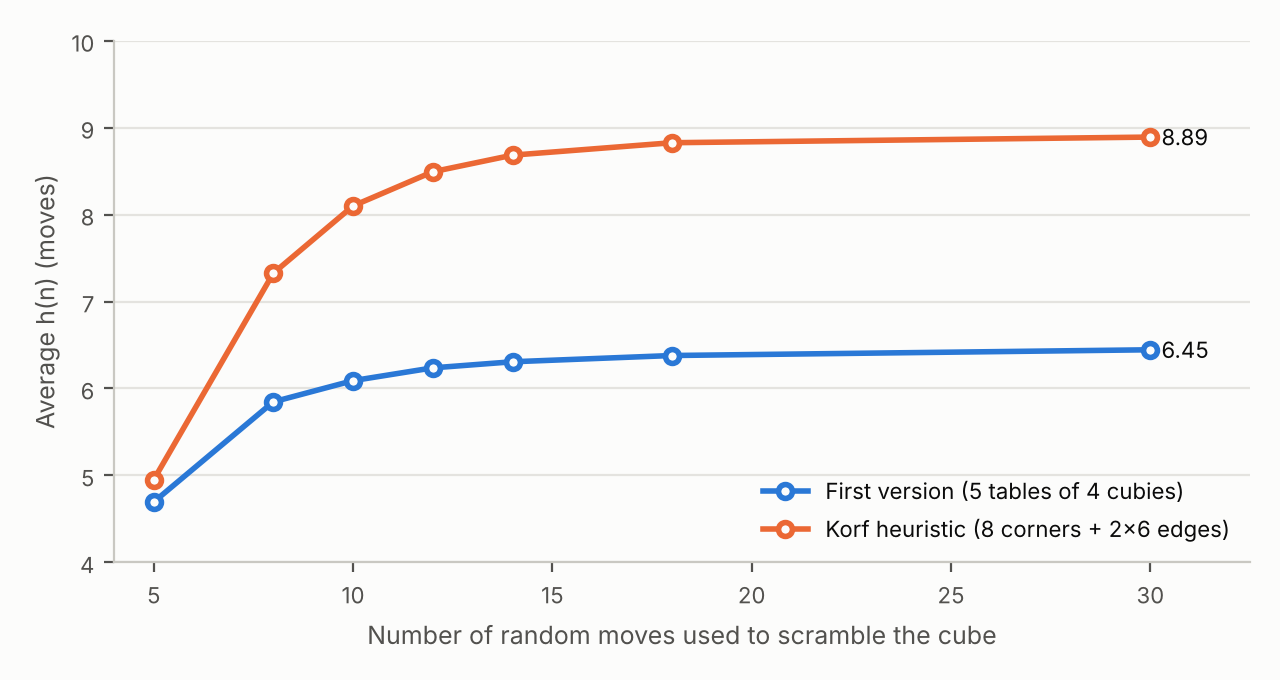
\includegraphics[width=\linewidth]{heuristic_strength.png}
        \captionof{figure}{Average value of $h$ for random cubes scrambled with different numbers of moves (20,000 cubes per point). Higher is better, as long as it is admissible.}
        \label{fig:hstrength}
    \end{minipage}
\end{center}

\subsubsection{Implementation details}
\begin{itemize}
    \item \textbf{Index of a table.} A pattern is converted to a number: the positions of the tracked cubies are encoded as a permutation number (Lehmer code), and the twists or flips of the cubies as a number in base 3 (corners) or base 2 (edges).
    \item \textbf{Open list.} Since every move costs 1, $f$ is always a small integer. Instead of a heap, the open list of our C++ A* is an array of lists, one list for every value of $f$. Inside a list, the newest node is expanded first (it has a larger $g$, so it is closer to the goal).
    \item \textbf{Redundant moves.} A face is never turned twice in a row, because two consecutive turns of the same face are always equal to one single move.
    \item \textbf{Memory.} Korf used IDA* \cite{korf1985}, a version that needs almost no memory, because A* stores every node it generates. We keep A* because it is the algorithm requested in this project, so we expect that for the deepest scrambles the memory of the cluster will be the limit; this will be analyzed in the Results.
\end{itemize}
   inside \section{Development}.
%  Bibliography: see references_ieee.tex (keys used here: aima3, hart1968, korf1997, culberson1998,
%  felner2004, holte2006, rokicki2013, cube20, korf1985, patel2014)
% =============================================================================

\subsection{The heuristic of A*}
\label{sec:heuristic}

\subsubsection{What A* needs from a heuristic}
A* expands first the node with the smallest value
\begin{equation}
    f(n) = g(n) + h(n),
\end{equation}
where $g(n)$ is the number of moves already made to reach $n$ and $h(n)$ is an estimation of the moves that are still missing to reach the solved cube \cite{aima3, hart1968}. A good introduction with visual examples can be found in \cite{patel2014}. The quality of $h$ decides how many nodes A* has to visit, and for the Rubik's Cube this is critical: the cube has $43{,}252{,}003{,}274{,}489{,}856{,}000$ reachable states \cite{korf1997, cube20}, every state has 18 possible moves (quarter and half turns of the six faces), and even the hardest cubes need 20 moves \cite{rokicki2013}.

Two properties are important \cite[pp.~94--95]{aima3}:
\begin{itemize}
    \item \textbf{Admissible:} $h(n) \le h^{*}(n)$, where $h^{*}(n)$ is the real number of moves needed from $n$. The heuristic never overestimates.
    \item \textbf{Consistent:} $h(n) \le c(n,a,n') + h(n')$ for every move $a$ that goes from $n$ to $n'$. Since every move costs $c = 1$, this means that $h$ changes at most by 1 after one move.
\end{itemize}
If $h$ is consistent (and therefore admissible), A* returns a shortest solution and a state never needs to be expanded twice \cite[p.~95]{aima3}. We need both properties in our program.

\subsubsection{First version of the heuristic and its problems}
Our first Python implementation used five small tables (explained below), each one storing information about only 4 cubies: two tables for 4 corners ($8\cdot7\cdot6\cdot5\cdot3^4 = 136{,}080$ states each) and three tables for 4 edges ($12\cdot11\cdot10\cdot9\cdot2^4 = 190{,}080$ states each), 842,400 entries in total. The heuristic was the maximum of the five values. It was correct, but it had two problems:
\begin{enumerate}
    \item \textbf{It is weak.} Each table ignores 8 of the 20 movable cubies, so its values are small. We measured the average value of $h$ over 20,000 random cubes and obtained only $6.45$ moves, while a typical random cube needs 17 or 18 moves \cite{cube20}. A weak heuristic makes A* expand a huge number of nodes.
    \item \textbf{It was built for 12 moves.} In the Python version only quarter turns existed. In this project we also use half turns ($F2$, $U2$, \dots), so there are 18 moves. A table built with quarter turns counts a half turn as 2 moves, so it can overestimate when the search counts it as 1 move, and the heuristic would stop being admissible. Every table must be built with exactly the same moves as the search.
\end{enumerate}

\subsubsection{Pattern databases}
The idea of a \textit{pattern database} (PDB) was introduced by Culberson and Schaeffer \cite{culberson1998} and it is also explained in our course book \cite[p.~106]{aima3}. We choose a part of the problem (for example, only the 8 corners of the cube and we ignore the edges). The number of moves needed to solve only that part can never be larger than the number of moves needed to solve the whole cube, so it is an admissible heuristic. Since that smaller problem has few states, we can solve \emph{all} its states in advance and save the answers in a table. During A*, computing $h(n)$ is only one table look-up.

The table is built with a breadth-first search that starts at the solved cube and applies the 18 moves again and again. The first time that the search reaches an arrangement of the pieces, the current depth is the distance of that arrangement to the solved state (the moves can be undone, so the distance from the solved cube is the same as the distance to it).

\subsubsection{Heuristic selected: 8 corners and two groups of 6 edges}
For the final version we use the heuristic of Korf \cite{korf1997}, who solved random cubes optimally with it. It uses three pattern databases:
\begin{enumerate}
    \item all 8 corners: $8! \cdot 3^7 = 88{,}179{,}840$ entries (the last corner twist is determined by the other seven, hence $3^7$);
    \item 6 edges (the first six edge cubies): $\frac{12!}{6!} \cdot 2^6 = 42{,}577{,}920$ entries;
    \item the other 6 edges: also $42{,}577{,}920$ entries.
\end{enumerate}
The heuristic is the maximum of the three values:
\begin{equation}
    h(n) = \max\bigl(h_{\text{corners}}(n),\; h_{\text{edges A}}(n),\; h_{\text{edges B}}(n)\bigr).
\end{equation}
Table~\ref{tab:pdb} shows the tables. Korf stored 4 bits per entry (82 MB in total); to keep our code simple we store one byte per entry (173 MB), which is small for our cluster. The tables are built once (about 12 seconds in our tests with 2 threads) and they are saved in a file for the next executions. As a check of our implementation, the average of the corner table is $8.764$, exactly the value reported by Korf \cite{korf1997}.

\begin{table}[H]
    \centering
    \renewcommand{\arraystretch}{1.3}
    \begin{tabular}{lrrrr}
        \toprule
        \textbf{Table} & \textbf{Entries} & \textbf{Memory} & \textbf{Average $h$} & \textbf{Max.\ $h$} \\
        \midrule
        8 corners          & 88,179,840 & 88.2 MB & 8.764 & 11 \\
        6 edges, set A     & 42,577,920 & 42.6 MB & 7.623 & 10 \\
        6 edges, set B     & 42,577,920 & 42.6 MB & 7.614 & 10 \\
        \bottomrule
    \end{tabular}
    \caption{Pattern databases used by A* (averages over all the entries of each table, measured with our program; Korf reports 8.764 for the corners and 7.668 for his 6-edge table \cite{korf1997}).}
    \label{tab:pdb}
\end{table}

\paragraph{Why the maximum and not the sum.} It would be tempting to add the three values to get a bigger heuristic, but this is not admissible for the cube: one turn of a face moves 4 corners \emph{and} 4 edges at the same time, so the same move would be counted in two tables. Adding values is only valid when the tables count different moves, as in additive pattern databases for sliding-tile puzzles \cite{felner2004}; the book also remarks that this does not work for the Rubik's Cube \cite[p.~107]{aima3}. Korf states that the only admissible way to combine corner and edge tables is to take the maximum \cite{korf1997}, and Holte et al.\ studied experimentally the use of several tables with the maximum \cite{holte2006}. We can also prove that the maximum keeps the two properties. Let $h_1, \dots, h_k$ be admissible and consistent heuristics and $h = \max_i h_i$:
\begin{itemize}
    \item \textit{Admissible:} for each $i$, $h_i(n) \le h^{*}(n)$, so $\max_i h_i(n) \le h^{*}(n)$.
    \item \textit{Consistent:} for each $i$, $h_i(n) \le 1 + h_i(n') \le 1 + h(n')$. Taking the maximum over $i$ on the left side gives $h(n) \le 1 + h(n')$.
\end{itemize}
Each table is itself consistent because it is the exact distance in a smaller version of the same puzzle, where one real move changes the pattern by at most one move. Our program also checks both properties in a self-test with thousands of random cubes.

\paragraph{How much better is it?} Figure~\ref{fig:hstrength} compares the average value of $h$ of the first version and of the final version over 20,000 random cubes for different scramble lengths. For a completely mixed cube the average goes from $6.45$ to $8.89$ moves (Korf reports $8.878$ \cite{korf1997}). It seems a small difference, but A* has to visit all the nodes with $f(n) = g(n) + h(n)$ smaller than the solution length, and the number of nodes grows exponentially with the depth, so every extra move of the heuristic removes a large part of the search. Korf also observed that the running time goes down approximately in proportion to the size of the tables \cite{korf1997}; our final tables have $173{,}335{,}680$ entries, about 206 times more than the 842,400 entries of the first version.

\begin{center}
    \begin{minipage}{0.9\textwidth}
        \centering
        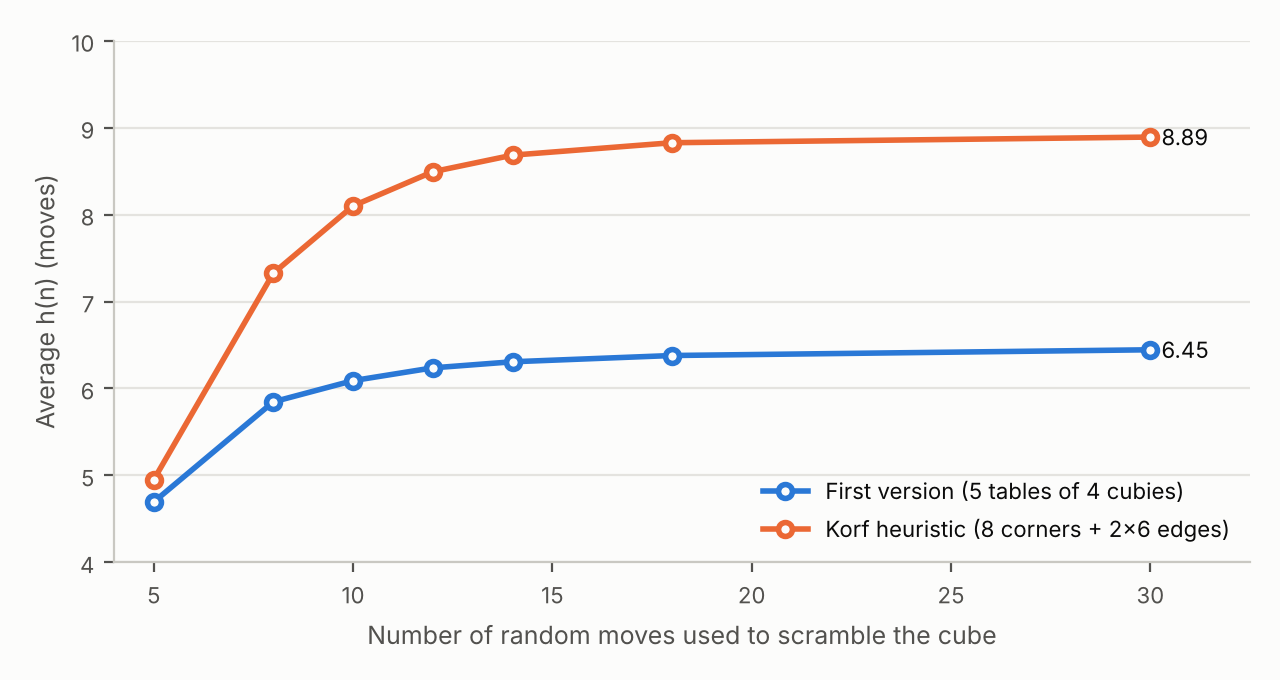
\includegraphics[width=\linewidth]{heuristic_strength.png}
        \captionof{figure}{Average value of $h$ for random cubes scrambled with different numbers of moves (20,000 cubes per point). Higher is better, as long as it is admissible.}
        \label{fig:hstrength}
    \end{minipage}
\end{center}

\subsubsection{Implementation details}
\begin{itemize}
    \item \textbf{Index of a table.} A pattern is converted to a number: the positions of the tracked cubies are encoded as a permutation number (Lehmer code), and the twists or flips of the cubies as a number in base 3 (corners) or base 2 (edges).
    \item \textbf{Open list.} Since every move costs 1, $f$ is always a small integer. Instead of a heap, the open list of our C++ A* is an array of lists, one list for every value of $f$. Inside a list, the newest node is expanded first (it has a larger $g$, so it is closer to the goal).
    \item \textbf{Redundant moves.} A face is never turned twice in a row, because two consecutive turns of the same face are always equal to one single move.
    \item \textbf{Memory.} Korf used IDA* \cite{korf1985}, a version that needs almost no memory, because A* stores every node it generates. We keep A* because it is the algorithm requested in this project, so we expect that for the deepest scrambles the memory of the cluster will be the limit; this will be analyzed in the Results.
\end{itemize}
   inside \section{Development}.
%  Bibliography: see references_ieee.tex (keys used here: aima3, hart1968, korf1997, culberson1998,
%  felner2004, holte2006, rokicki2013, cube20, korf1985, patel2014)
% =============================================================================

\subsection{The heuristic of A*}
\label{sec:heuristic}

\subsubsection{What A* needs from a heuristic}
A* expands first the node with the smallest value
\begin{equation}
    f(n) = g(n) + h(n),
\end{equation}
where $g(n)$ is the number of moves already made to reach $n$ and $h(n)$ is an estimation of the moves that are still missing to reach the solved cube \cite{aima3, hart1968}. A good introduction with visual examples can be found in \cite{patel2014}. The quality of $h$ decides how many nodes A* has to visit, and for the Rubik's Cube this is critical: the cube has $43{,}252{,}003{,}274{,}489{,}856{,}000$ reachable states \cite{korf1997, cube20}, every state has 18 possible moves (quarter and half turns of the six faces), and even the hardest cubes need 20 moves \cite{rokicki2013}.

Two properties are important \cite[pp.~94--95]{aima3}:
\begin{itemize}
    \item \textbf{Admissible:} $h(n) \le h^{*}(n)$, where $h^{*}(n)$ is the real number of moves needed from $n$. The heuristic never overestimates.
    \item \textbf{Consistent:} $h(n) \le c(n,a,n') + h(n')$ for every move $a$ that goes from $n$ to $n'$. Since every move costs $c = 1$, this means that $h$ changes at most by 1 after one move.
\end{itemize}
If $h$ is consistent (and therefore admissible), A* returns a shortest solution and a state never needs to be expanded twice \cite[p.~95]{aima3}. We need both properties in our program.

\subsubsection{First version of the heuristic and its problems}
Our first Python implementation used five small tables (explained below), each one storing information about only 4 cubies: two tables for 4 corners ($8\cdot7\cdot6\cdot5\cdot3^4 = 136{,}080$ states each) and three tables for 4 edges ($12\cdot11\cdot10\cdot9\cdot2^4 = 190{,}080$ states each), 842,400 entries in total. The heuristic was the maximum of the five values. It was correct, but it had two problems:
\begin{enumerate}
    \item \textbf{It is weak.} Each table ignores 8 of the 20 movable cubies, so its values are small. We measured the average value of $h$ over 20,000 random cubes and obtained only $6.45$ moves, while a typical random cube needs 17 or 18 moves \cite{cube20}. A weak heuristic makes A* expand a huge number of nodes.
    \item \textbf{It was built for 12 moves.} In the Python version only quarter turns existed. In this project we also use half turns ($F2$, $U2$, \dots), so there are 18 moves. A table built with quarter turns counts a half turn as 2 moves, so it can overestimate when the search counts it as 1 move, and the heuristic would stop being admissible. Every table must be built with exactly the same moves as the search.
\end{enumerate}

\subsubsection{Pattern databases}
The idea of a \textit{pattern database} (PDB) was introduced by Culberson and Schaeffer \cite{culberson1998} and it is also explained in our course book \cite[p.~106]{aima3}. We choose a part of the problem (for example, only the 8 corners of the cube and we ignore the edges). The number of moves needed to solve only that part can never be larger than the number of moves needed to solve the whole cube, so it is an admissible heuristic. Since that smaller problem has few states, we can solve \emph{all} its states in advance and save the answers in a table. During A*, computing $h(n)$ is only one table look-up.

The table is built with a breadth-first search that starts at the solved cube and applies the 18 moves again and again. The first time that the search reaches an arrangement of the pieces, the current depth is the distance of that arrangement to the solved state (the moves can be undone, so the distance from the solved cube is the same as the distance to it).

\subsubsection{Heuristic selected: 8 corners and two groups of 6 edges}
For the final version we use the heuristic of Korf \cite{korf1997}, who solved random cubes optimally with it. It uses three pattern databases:
\begin{enumerate}
    \item all 8 corners: $8! \cdot 3^7 = 88{,}179{,}840$ entries (the last corner twist is determined by the other seven, hence $3^7$);
    \item 6 edges (the first six edge cubies): $\frac{12!}{6!} \cdot 2^6 = 42{,}577{,}920$ entries;
    \item the other 6 edges: also $42{,}577{,}920$ entries.
\end{enumerate}
The heuristic is the maximum of the three values:
\begin{equation}
    h(n) = \max\bigl(h_{\text{corners}}(n),\; h_{\text{edges A}}(n),\; h_{\text{edges B}}(n)\bigr).
\end{equation}
Table~\ref{tab:pdb} shows the tables. Korf stored 4 bits per entry (82 MB in total); to keep our code simple we store one byte per entry (173 MB), which is small for our cluster. The tables are built once (about 12 seconds in our tests with 2 threads) and they are saved in a file for the next executions. As a check of our implementation, the average of the corner table is $8.764$, exactly the value reported by Korf \cite{korf1997}.

\begin{table}[H]
    \centering
    \renewcommand{\arraystretch}{1.3}
    \begin{tabular}{lrrrr}
        \toprule
        \textbf{Table} & \textbf{Entries} & \textbf{Memory} & \textbf{Average $h$} & \textbf{Max.\ $h$} \\
        \midrule
        8 corners          & 88,179,840 & 88.2 MB & 8.764 & 11 \\
        6 edges, set A     & 42,577,920 & 42.6 MB & 7.623 & 10 \\
        6 edges, set B     & 42,577,920 & 42.6 MB & 7.614 & 10 \\
        \bottomrule
    \end{tabular}
    \caption{Pattern databases used by A* (averages over all the entries of each table, measured with our program; Korf reports 8.764 for the corners and 7.668 for his 6-edge table \cite{korf1997}).}
    \label{tab:pdb}
\end{table}

\paragraph{Why the maximum and not the sum.} It would be tempting to add the three values to get a bigger heuristic, but this is not admissible for the cube: one turn of a face moves 4 corners \emph{and} 4 edges at the same time, so the same move would be counted in two tables. Adding values is only valid when the tables count different moves, as in additive pattern databases for sliding-tile puzzles \cite{felner2004}; the book also remarks that this does not work for the Rubik's Cube \cite[p.~107]{aima3}. Korf states that the only admissible way to combine corner and edge tables is to take the maximum \cite{korf1997}, and Holte et al.\ studied experimentally the use of several tables with the maximum \cite{holte2006}. We can also prove that the maximum keeps the two properties. Let $h_1, \dots, h_k$ be admissible and consistent heuristics and $h = \max_i h_i$:
\begin{itemize}
    \item \textit{Admissible:} for each $i$, $h_i(n) \le h^{*}(n)$, so $\max_i h_i(n) \le h^{*}(n)$.
    \item \textit{Consistent:} for each $i$, $h_i(n) \le 1 + h_i(n') \le 1 + h(n')$. Taking the maximum over $i$ on the left side gives $h(n) \le 1 + h(n')$.
\end{itemize}
Each table is itself consistent because it is the exact distance in a smaller version of the same puzzle, where one real move changes the pattern by at most one move. Our program also checks both properties in a self-test with thousands of random cubes.

\paragraph{How much better is it?} Figure~\ref{fig:hstrength} compares the average value of $h$ of the first version and of the final version over 20,000 random cubes for different scramble lengths. For a completely mixed cube the average goes from $6.45$ to $8.89$ moves (Korf reports $8.878$ \cite{korf1997}). It seems a small difference, but A* has to visit all the nodes with $f(n) = g(n) + h(n)$ smaller than the solution length, and the number of nodes grows exponentially with the depth, so every extra move of the heuristic removes a large part of the search. Korf also observed that the running time goes down approximately in proportion to the size of the tables \cite{korf1997}; our final tables have $173{,}335{,}680$ entries, about 206 times more than the 842,400 entries of the first version.

\begin{center}
    \begin{minipage}{0.9\textwidth}
        \centering
        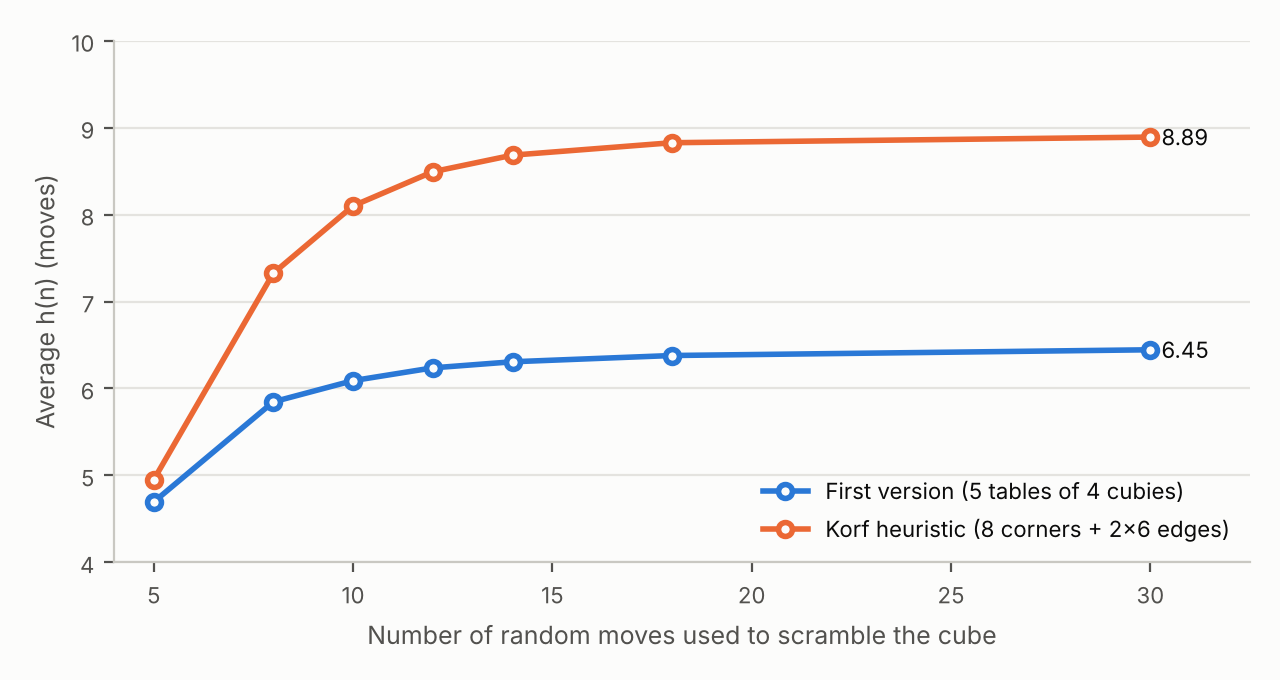
\includegraphics[width=\linewidth]{heuristic_strength.png}
        \captionof{figure}{Average value of $h$ for random cubes scrambled with different numbers of moves (20,000 cubes per point). Higher is better, as long as it is admissible.}
        \label{fig:hstrength}
    \end{minipage}
\end{center}

\subsubsection{Implementation details}
\begin{itemize}
    \item \textbf{Index of a table.} A pattern is converted to a number: the positions of the tracked cubies are encoded as a permutation number (Lehmer code), and the twists or flips of the cubies as a number in base 3 (corners) or base 2 (edges).
    \item \textbf{Open list.} Since every move costs 1, $f$ is always a small integer. Instead of a heap, the open list of our C++ A* is an array of lists, one list for every value of $f$. Inside a list, the newest node is expanded first (it has a larger $g$, so it is closer to the goal).
    \item \textbf{Redundant moves.} A face is never turned twice in a row, because two consecutive turns of the same face are always equal to one single move.
    \item \textbf{Memory.} Korf used IDA* \cite{korf1985}, a version that needs almost no memory, because A* stores every node it generates. We keep A* because it is the algorithm requested in this project, so we expect that for the deepest scrambles the memory of the cluster will be the limit; this will be analyzed in the Results.
\end{itemize}
